\documentclass[10pt]{article}
\usepackage[top = 0.75in, bottom = 1.0in, left = 1.0in, right = 1.0in]{geometry}
\usepackage{float}
\usepackage{amsmath}
\usepackage{graphicx}
\usepackage{indentfirst}
\graphicspath{ {../figures/} }
\title{CS 418 Final Project}
\date{December 2, 2019}
\author {Manasa Kandimalla, Shyam Patel, Carlos Antonio McNulty}
\begin{document}
\maketitle

\section*{1. Problem Selection}

For our final project, we would like to solve the problem: which personality traits (e.g., neuroticism, extraversion, openness to experience, agreeableness, conscientiousness, impulsiveness and sensation) and other factors (e.g., age, gender and education) make one susceptible to the usage of various illegal drugs. These drugs include amphetamines, amyl nitrite, benzodiazepine, cannabis, cocaine, crack, ecstasy, heroin, ketamine, legal highs, LSD, methadone, mushrooms and volatile substance abuse (VSA).


\section*{2. Data Collection}

The data for our project consists of a single dataset titled \textit{Drug consumption} donated to the UCI Machine Learning Repository in 2016. The original owners of the database are Elaine Fehrman, Vincent Egan and Evgeny M. Mirkes. The database contains records for 1,885 respondents. For each respondent, 12 attributes are known: measurements which include NEO-FFI-R (neuroticism, extraversion, openness to experience, agreeableness, and conscientiousness), BIS-11 (impulsivity), and ImpSS (sensation seeking), level of education, age, gender, country of residence and ethnicity. Each respondent also provided their usage for 18 legal and illegal drugs, including the fictitious drug Semeron. The 7 categories for drug usage consist of: (1) never used, (2) used over a decade ago, (3) used in the last decade, (4) used in the last year, (5) used in the last month, (6) used in the last week, and (7) used in the last day.

\section*{3. Data Preparation}

The provided dataset does not include a header. For ease of use with the Pandas library, we added a header. To allow us to perform some analysis of the dataset, we needed to convert the values in the dataset to something more interpretable. For instance, the values for male and female were provided as the values -0.48246 and 0.48246, respectively. We converted these into categorical variables, at least for the duration of our analysis. We also had to label encode the drug usage responses and one-hot encode the gender category for later use with classifiers. Second, the categories of drug usage (e.g., never used, used over a decade ago, used in the last decade, used in the last year, used in the last month, used in the last week, and used in the last day) were converted into integers, which was used to add a binary \textit{Drug User} variable that simply distinguishes between respondents who used any illegal drugs in the past and those who did not.

\section*{4. Data Exploration}

\begin{figure}[H]
\caption{Drug Usage}
\label{fig:drugs}
\centering
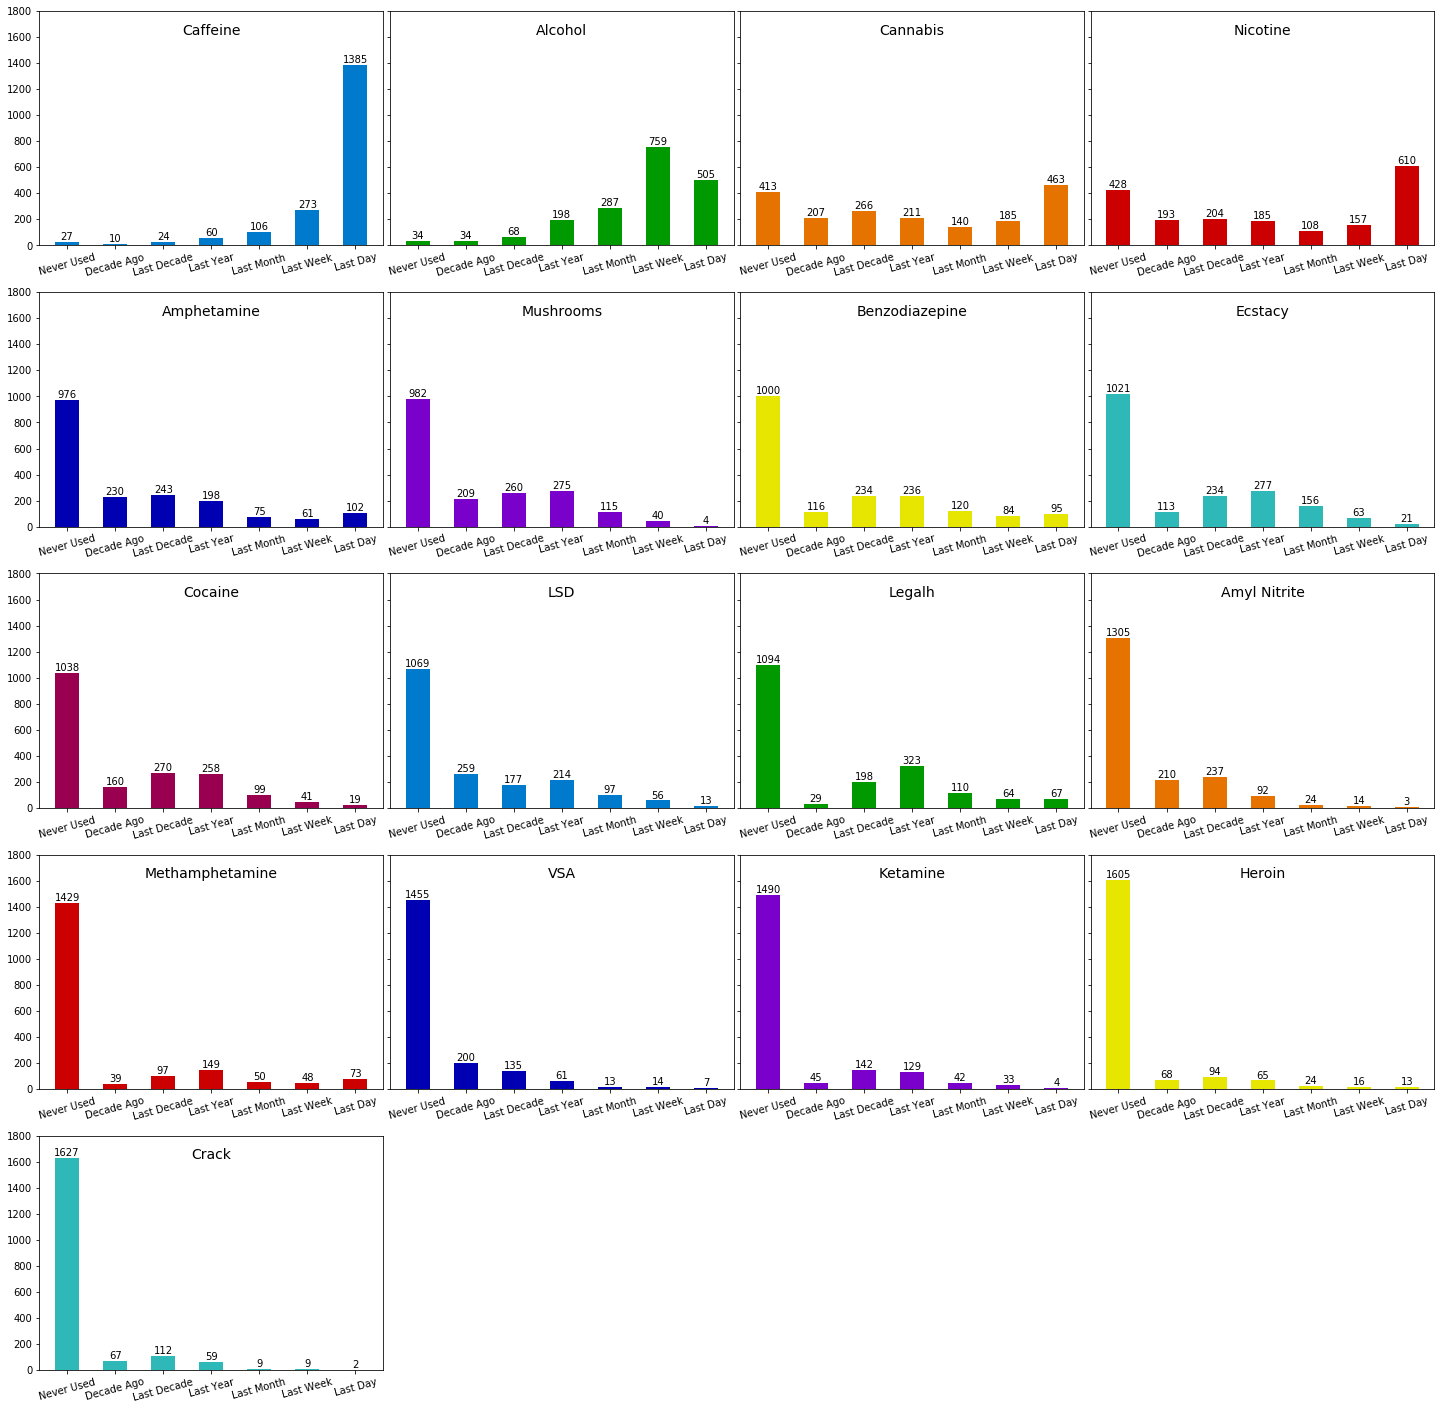
\includegraphics[scale=0.6]{drugs.png}
\end{figure}

In Figure \ref{fig:drugs}, we see all 17 drugs, ordered from most frequently to least frequently used, and their corresponding usage. The drugs used by the most respondents and those used most frequently are the class of legal drugs and cannabis. The most used illegal drug is cannabis with 1,472 total users, or about 78\% of respondents. For the remaining drugs usage declined sharply with the least used drug being crack. It had a total of 258 users, or about 13.7\% of respondents. Usage for most of the drugs in the dataset followed a normal distribution.


\begin{figure}[H]
\caption{Illegal Drug Usage by Personality Trait}
\label{fig:traits}
\centering
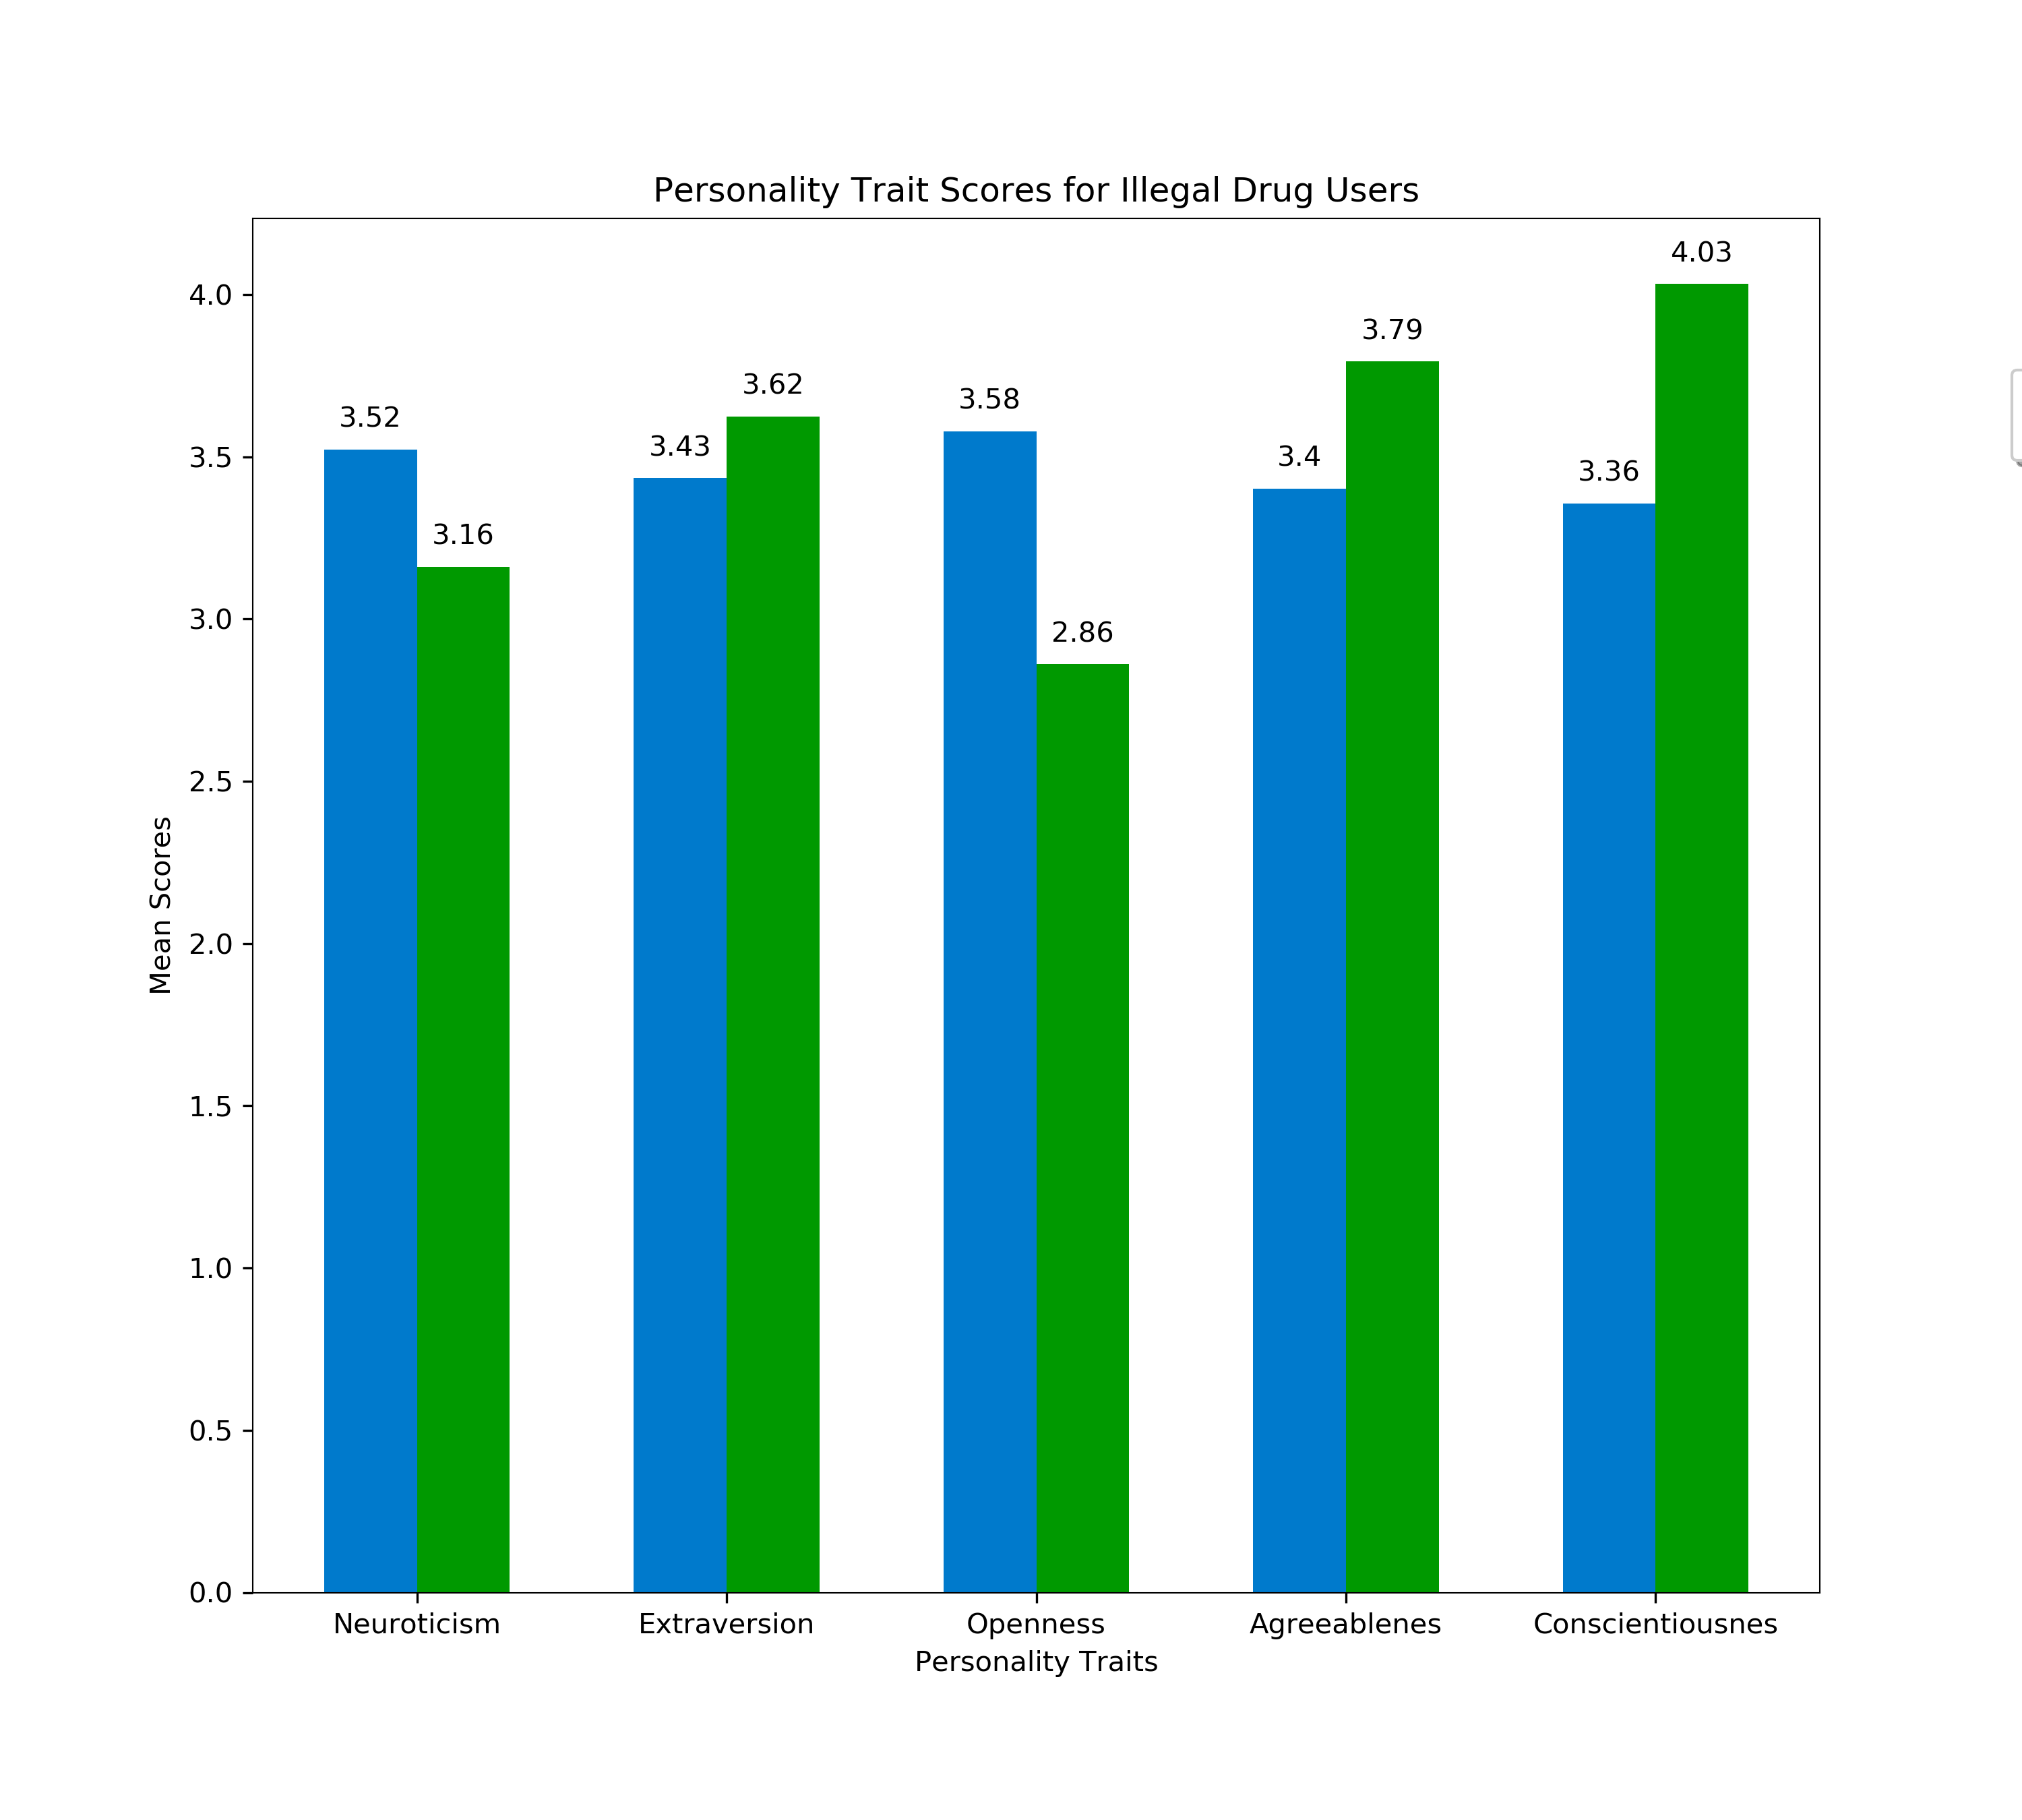
\includegraphics[scale=0.22]{traits.png}
\end{figure}

One of the primary focuses of our research was determining the relation between drug abuse and personality traits. We see in Figure \ref{fig:traits} that drug users had higher mean scores for both \textit{Neuroticism} and \textit{Openness}. These are both characteristics we might except from an average drug user. These users also scored lower on \textit{Extraversion}, \textit{Agreeableness}, and \textit{Conscientiousness}. We analyzed these differences and found them to be statistically significant. Our p-values reflect one-sided t-tests. The two alternative hypotheses for the one-sided tests are that the mean drug user score is greater than the non-user score, and that the mean is less. \textit{Neuroticism} and \textit{Openness} can be considered right-tailed t-tests and the remaining traits left-sided t-tests. These p-values can be seen below in Table \ref{fig:pvalues}.

\begin{table}[H]
\centering
\caption{t-statistics and p-values for Figure \ref{fig:traits}}
\label{fig:pvalues}
\begin{tabular}{|l|l|l|}
\hline
       & t-statistic         & p-value\\ \hline
Nscore & 6.3434   & 2.6924e-10  \\ \hline
Escore & -3.4179  & 0.0003  \\ \hline
Oscore & 13.2261  & 1.8035e-34 \\ \hline
Ascore & -6.3017  & 1.8286e-10 \\ \hline
Cscore & -12.7530 & 1.2412e-32 \\ \hline
\end{tabular}
\end{table}

In Figure \ref{fig:genders}, we see that the dataset had a total of 859 male drug users and 726 female drug users. The most notable difference between the two genders was in their frequency of usage, rather than in the total number of drug users. Of those who were surveyed, twice as many men than women responded that they had taken a drug in the last day. We also see that most male drug users had taken a drug in the last month, and most female drug users had taken a drug sometime in the last year or later. This might suggest that, while the number of women and men that use drugs is roughly equivalent, how frequently they use these drugs may differ drastically.


\begin{figure}[H]
\caption{Illegal Drug Usage and Frequency by Gender}
\label{fig:genders}
\centering
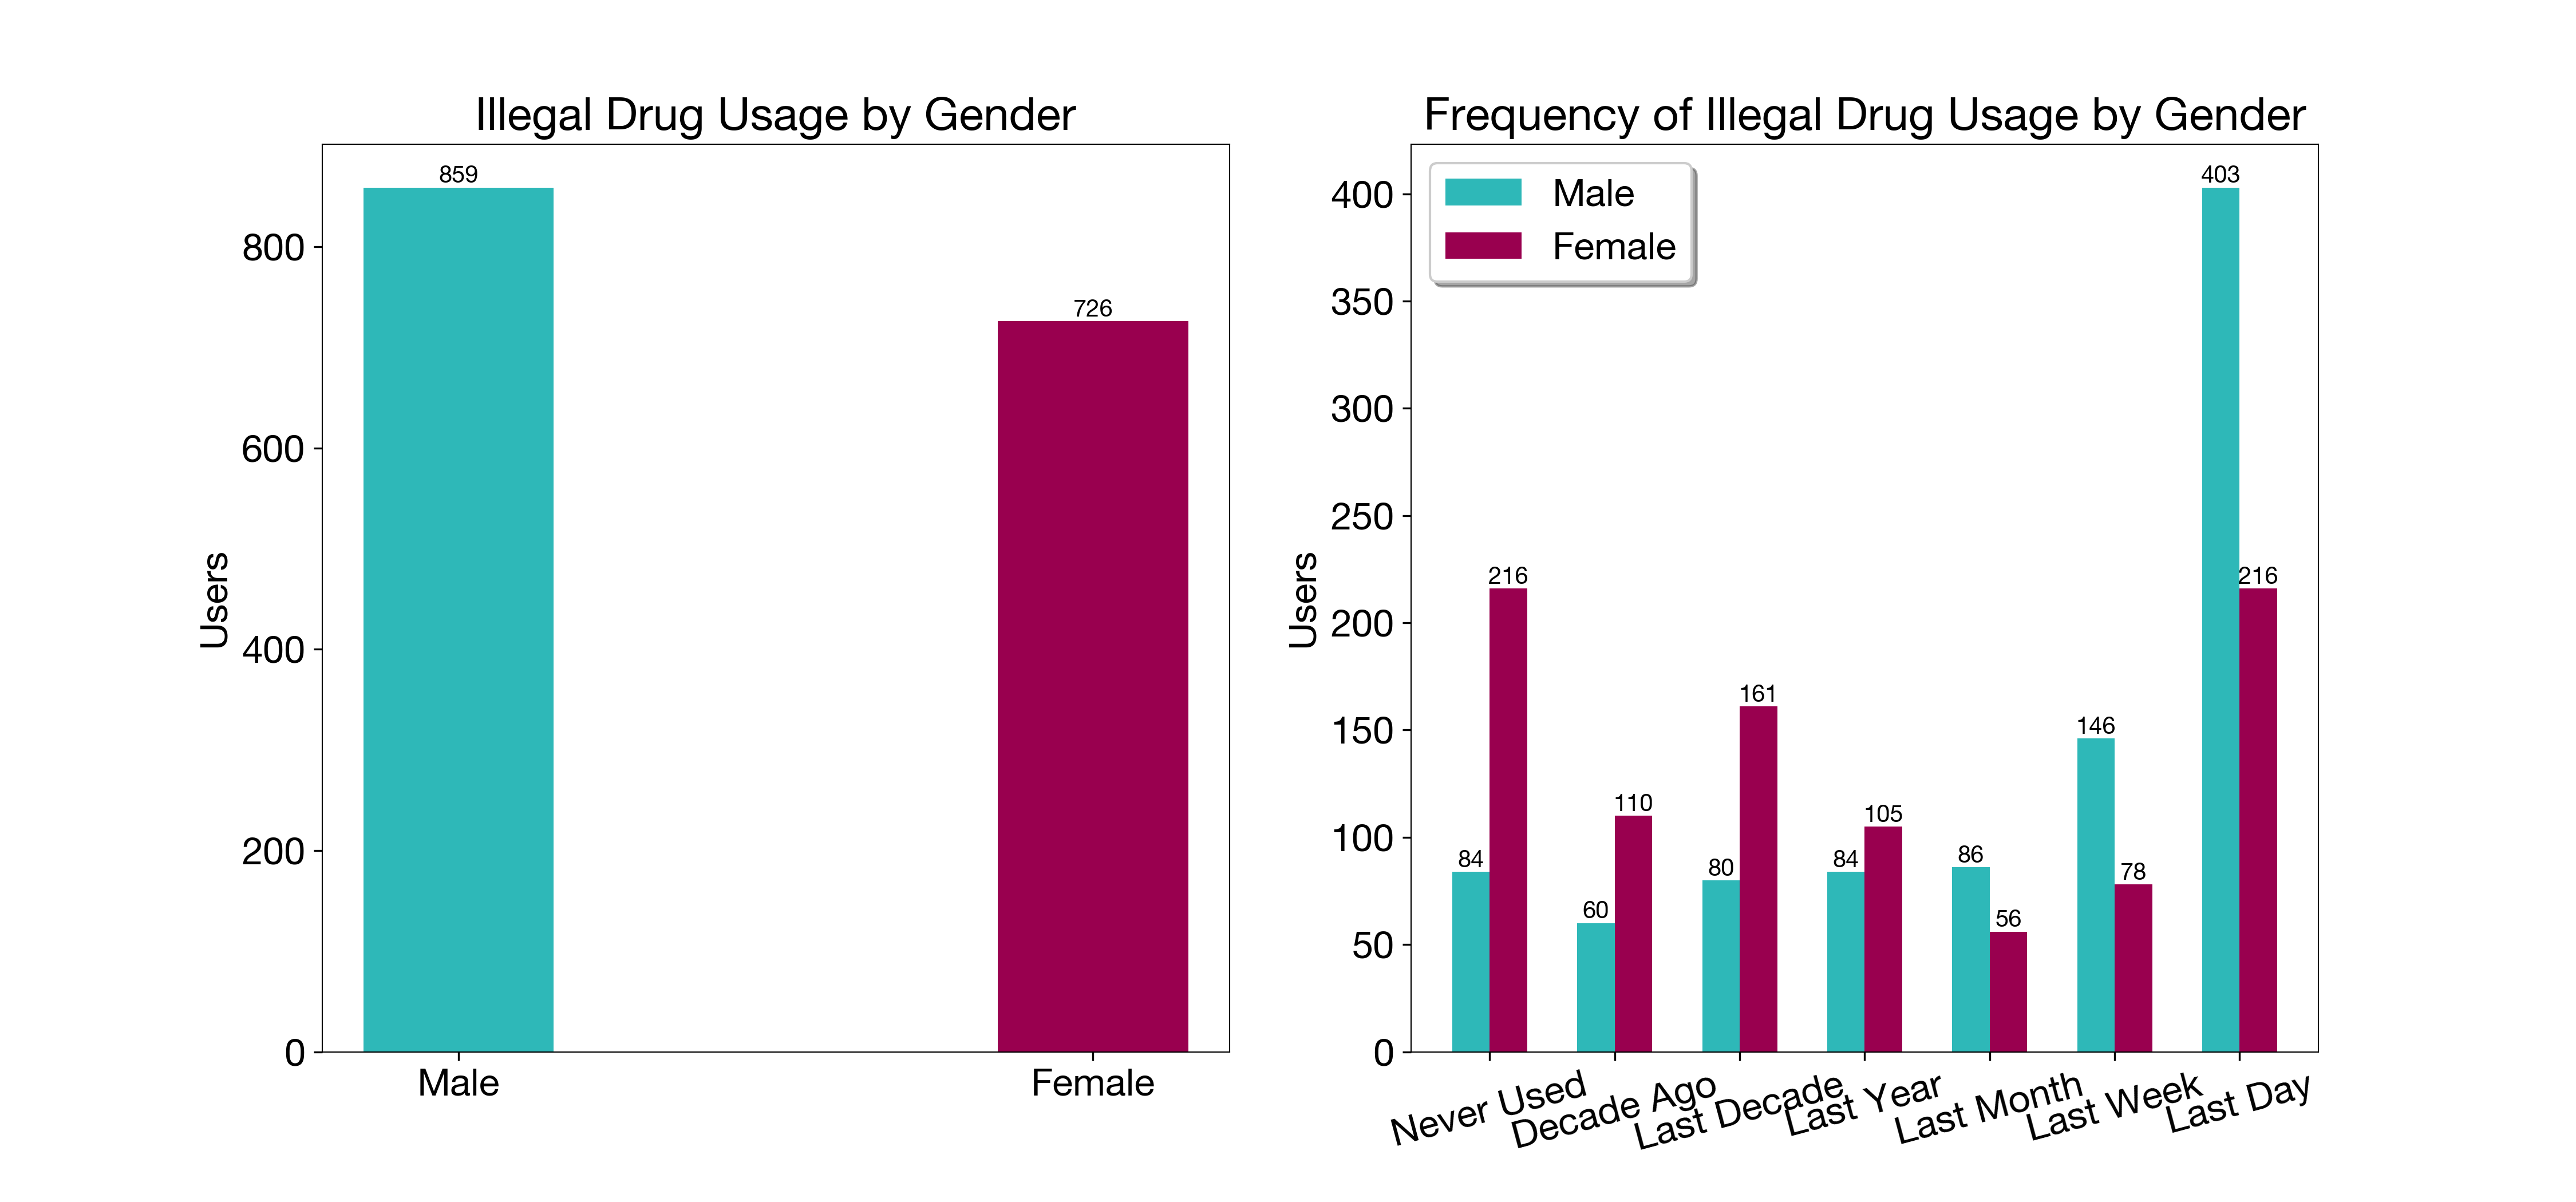
\includegraphics[scale=0.45]{gender_freq.png}
\end{figure}

In Figure \ref{fig:heatmap}, we constructed a Pearson correlation heatmap that depicts the correlation of independent variables with the output variable \textit{Drug User}. This enabled us to narrow the scope of independent variables and take only the subset of relevant features in our models. The features that are most highly correlated with \textit{Drug User} are: \textit{Country}, \textit{SS}, \textit{Cscore}, \textit{Oscore}, \textit{Impulsive}, and \textit{Age}.


\begin{figure}[H]
\caption{Heatmap of Correlation Matrix}
\label{fig:heatmap}
\centering
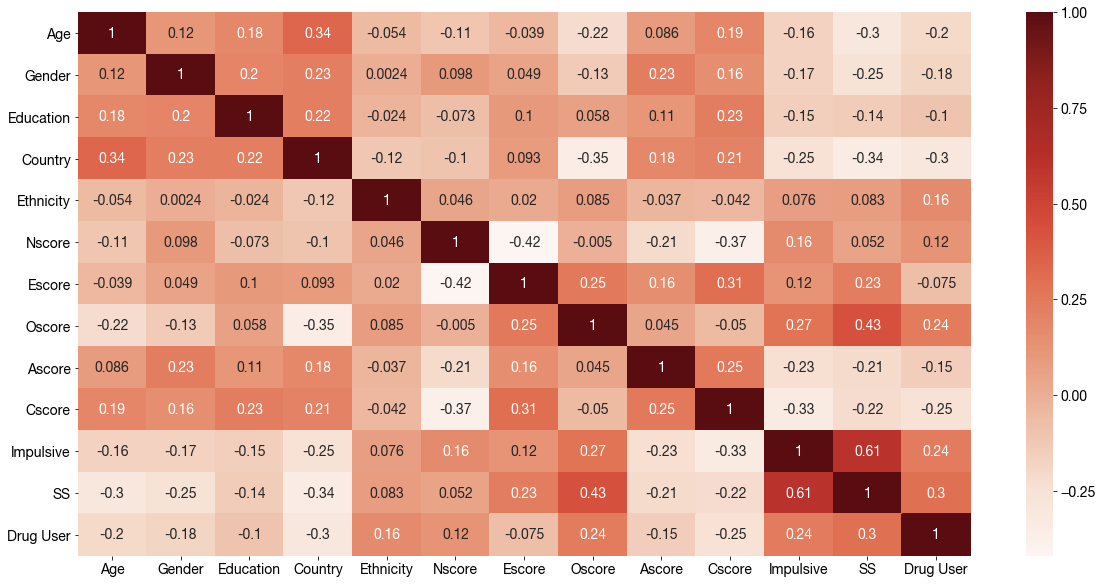
\includegraphics[scale=0.25]{heatmap.png}
\end{figure}

\section*{5. Data Modeling}

\subsection*{Decision Tree Classifier}

To begin our data modeling process that strives to classify people as drug users or non-users, we used a decision tree classifier. In order to select the independent variables that had a significant correlation with our output variable \textit{Drug User}, we used our Pearson correlation heatmap (see Figure \ref{fig:heatmap}) and selected features that had an absolute correlation value above the median correlation, 0.192. Using this, we successfully reduced the number of relevant variables from 12 to 6. In particular, only the features \textit{Age}, \textit{Country}, \textit{Oscore}, \textit{Cscore}, \textit{Impulsive} and \textit{SS} were found to be highly correlated with the output variable \textit{Drug User}.

Using the standardized training data, we used these relevant features to build a decision tree classifier. The resulting decision tree contains 475 nodes. The variable selected to split the root node of the decision tree is \textit{Country}. The decision tree has a large number of nodes, which may be evidence of overfitting. Using 10–fold cross validation, we found the mean accuracy of the model to be 79.0\% and the mean F1 score to be 87.4\%. To further assess the importance of each feature used in the model, we examined the \textit{Gini importance}, which is calculated as the decrease in node impurity weighted by the probability of reaching that node (e.g., the number of samples that reach the node, divided by the total number of samples). The features from most to least important are: (1) \textit{Cscore} with 0.243, (2) \textit{Oscore} with 0.203, (3) \textit{SS} with 0.173, (4) \textit{Country} with 0.135, (5) \textit{Age} with 0.131, and (6) \textit{Impulsive} with 0.115.

Next, we predicted the class labels for the test set using the decision tree classifier and plotted the corresponding confusion matrix (see Figure \ref{fig:conf_matrix_dt}). Overall, our model performed relatively well. 393 respondents who are actually drug users were correctly predicted to be users, and 32 respondents who are not drug users were correctly predicted to be non-users. However, 74 respondents who are actually drug users were incorrectly predicted to be non-users, and 67 respondents who are not drug users were incorrectly predicted to be users. As such, the decision tree classifier predicts drug usage with a precision (e.g., the proportion of respondents classified as drug users who are indeed users) of 85.4\% and a recall (e.g., the proportion of drug users who are classified correctly) of 84.2\%.

\begin{figure}[H]
\caption{Confusion Matrix of Decision Tree Classifier}
\label{fig:conf_matrix_dt}
\centering
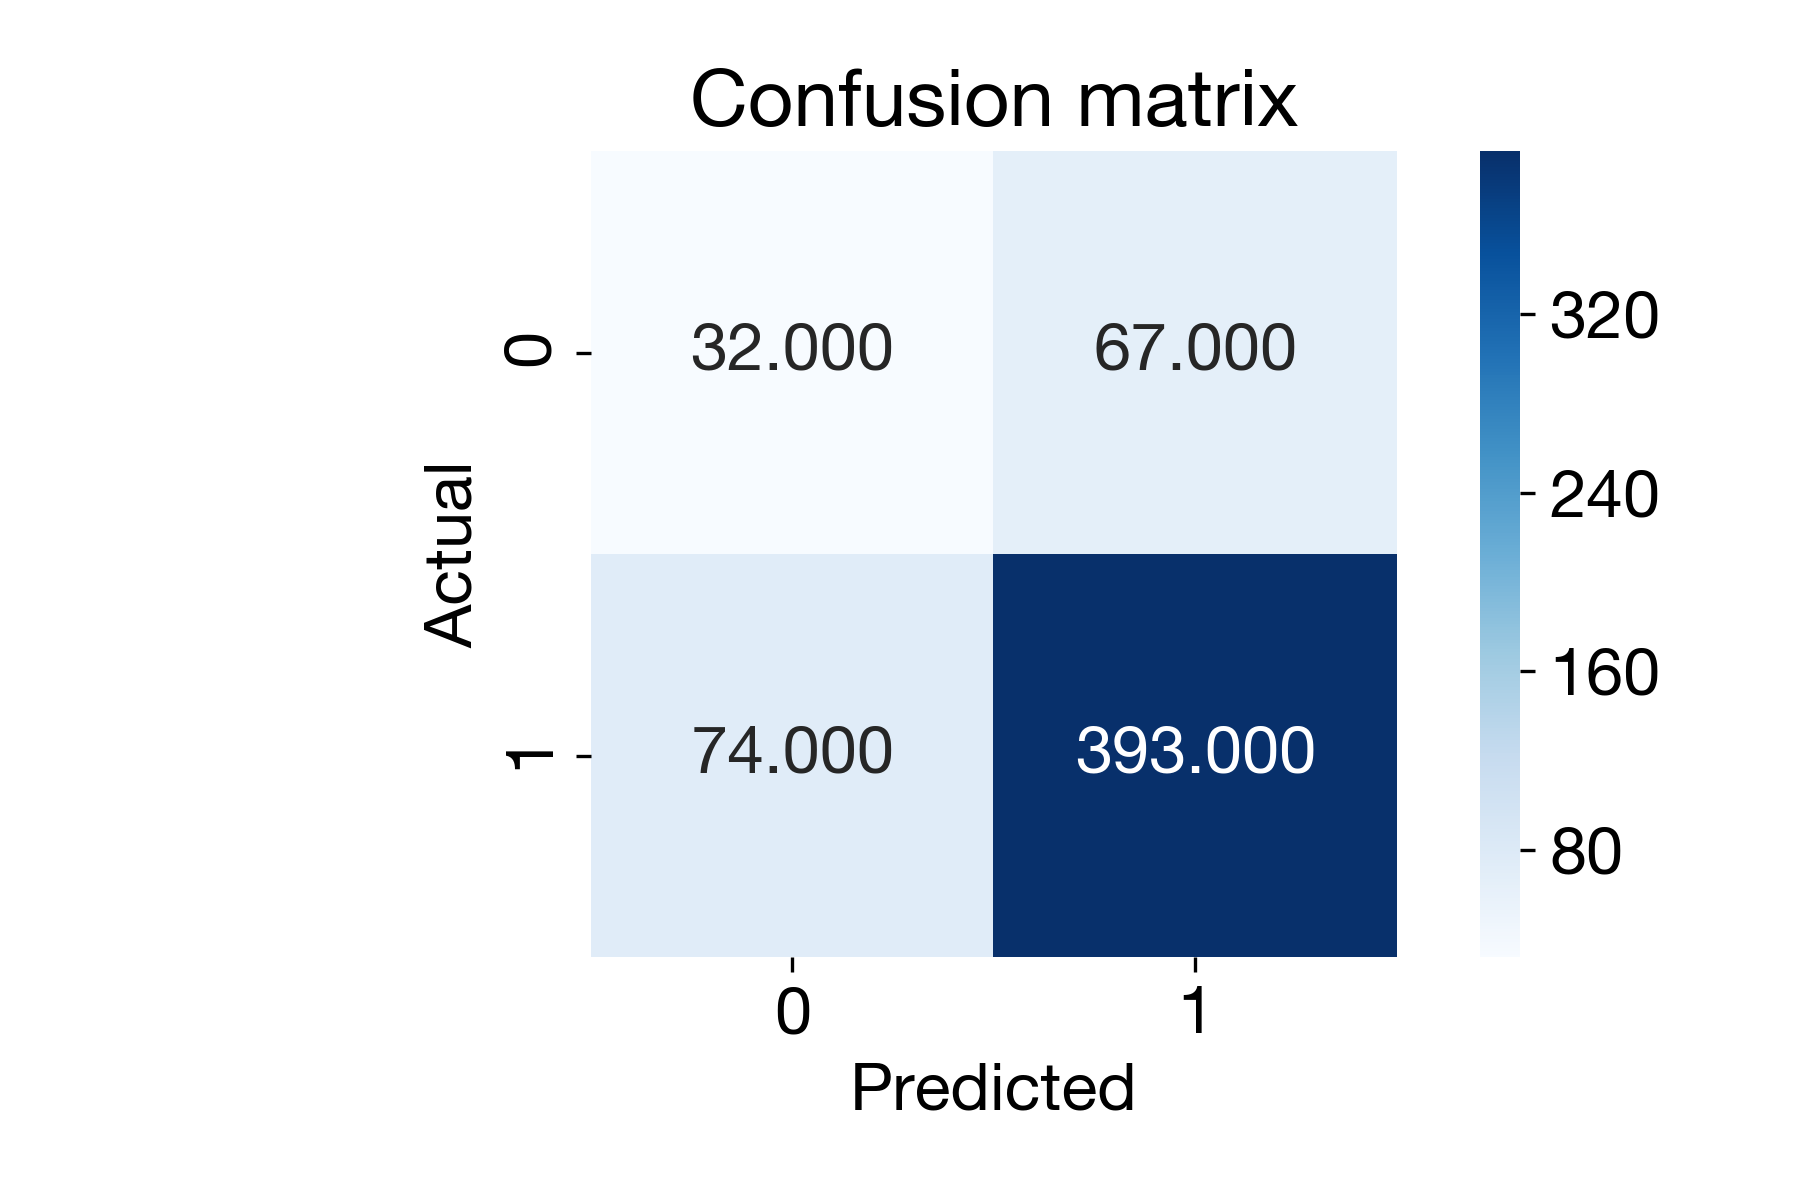
\includegraphics[scale=0.4]{conf_matrix_dt.png}
\end{figure}

\subsection*{k-Nearest Neighbors Classifier}

To determine whether or not we could improve upon the performance of the decision tree classifier, we used the same relevant features and standardized training data to build a k-nearest neighbors classifier. Using 10–fold cross validation, we found the mean accuracy of the k-nearest neighbors classifier to be 80.9\% and the mean F1 score to be 88.8\%, which indicates a higher performance than that of the decision tree classifier. We predicted the class labels for the test set using the k-nearest neighbors classifier and plotted the corresponding confusion matrix (see Figure \ref{fig:conf_matrix_knn}).

Our new model performed noticeably better. In particular, 423 respondents who are actually drug users were correctly predicted to be users, and 25 respondents who are not drug users were correctly predicted to be non-users. On the other hand, 44 respondents who are actually drug users were incorrectly predicted to be non-users, and 74 respondents who are not drug users were incorrectly predicted to be users. As such, the k-nearest neighbors classifier predicts drug usage with a precision of 85.1\% and a recall of 90.6\%. This is a slightly lower precision, but significantly higher recall than the decision tree classifier, which is explained by the higher number of FPs but lower number of FNs.

\begin{figure}[H]
\caption{Confusion Matrix of k-Nearest Neighbors Classifier}
\label{fig:conf_matrix_knn}
\centering
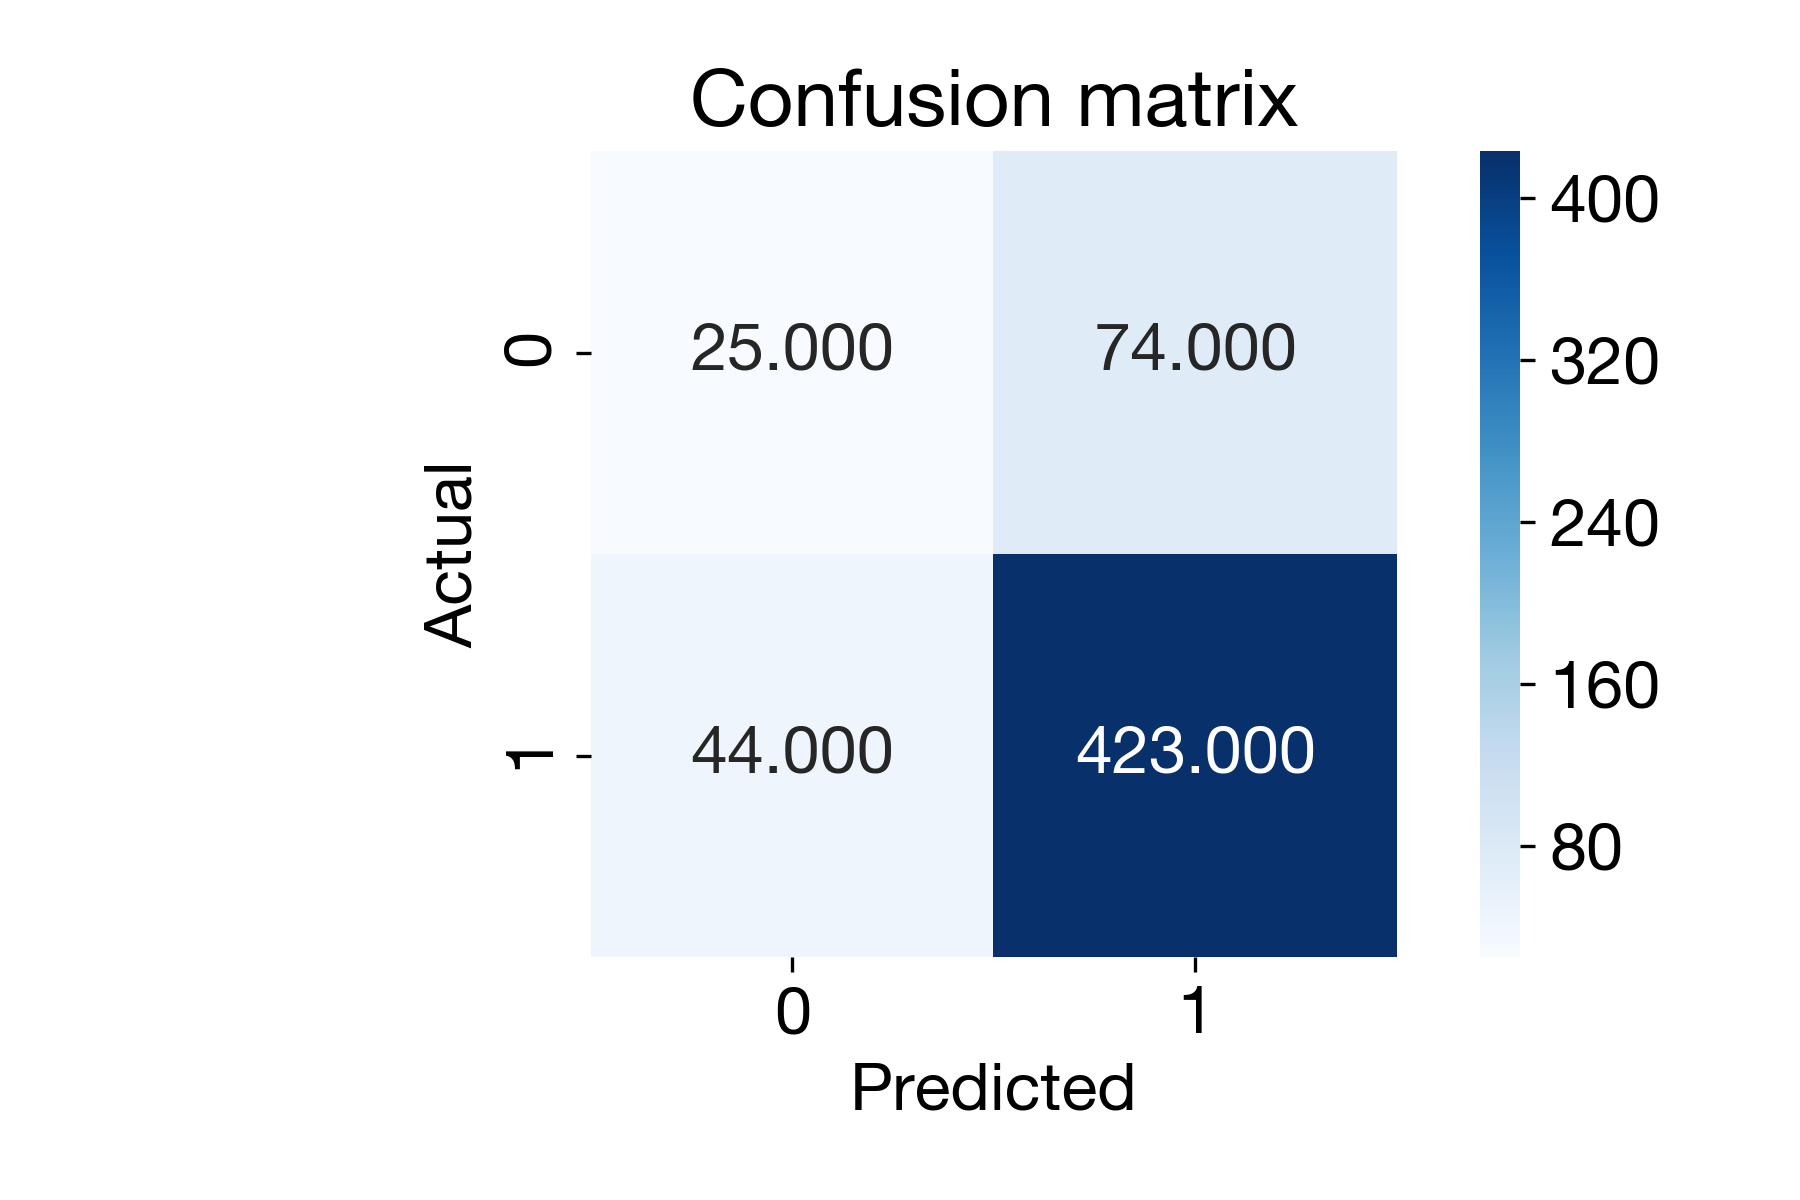
\includegraphics[scale=0.4]{conf_matrix_knn.png}
\end{figure}

\subsection*{Random Forest Classifier}


\subsubsection*{Feature Selection}

To select the features for our binary classifier we consulted the pearson correlation matrix in Figure \ref{fig:heatmap}. In addition a feature selection tool from sklearn was used that determines a models features importances and removes those that fall below a certain threshold. Our analysis indicated that the features that might be best for our model were Age, Education, Country, Nscore, Escore, Oscore, Ascore, Cscore, Impulsive, and SS. In Figure \ref{fig:genders} we saw there may be some distinction between the frequency of drug use for men and women, but no real difference in the total number of users. For a binary classifier the Gender variable would not be useful and when tested with cross validation showed no improvement.

\subsubsection*{Grid Search}

\begin{figure}[H]
\caption{Hyperparameter Tuning with Grid Search }
\label{fig:gridsearch}
\centering
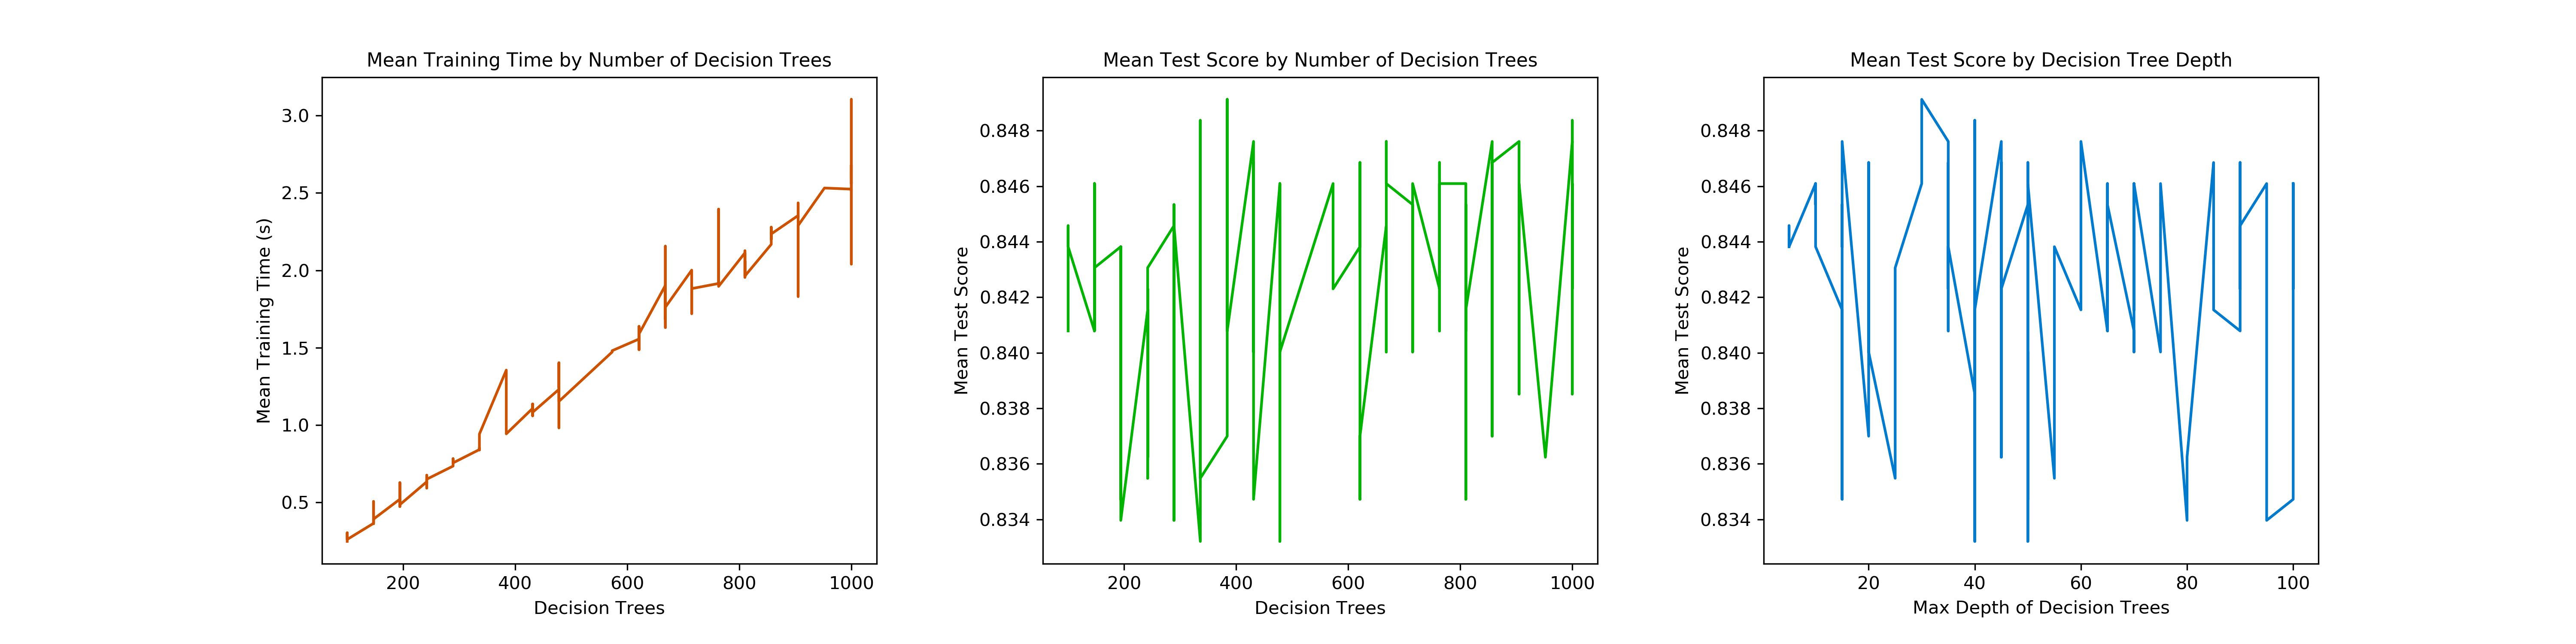
\includegraphics[scale=0.35]{gridsearch.png}
\end{figure}

We performed grid search on 30,240 random forests by varying the number of estimators and the configuration for the base estimators provided to each random forest. The exhaustive search then chose the best performing model when tested with 10-fold cross validation. This model had an F1 score of 0.844 and an accuracy of 0.913. When the model was applied to the test set it resulted in an accuracy of 0.827.

\subsection*{Clustering}

	For Clustering, we first converted all the values of drug variables into integers of range 0-6. For this data set, we do not have an actual class to compare the clusters against, so we could not use Rand Index as the evaluation metric for the clusters. We used the Silhouette Coefficient to measure the goodness of clusters. 
	We plotted the clusters with a total of 8 sets of features(All features, only illegal drugs, only non-illegal drugs, all drugs, all features excluding drugs, using personality traits,  personality traits with illegal drugs, personality traits with non-illegal drugs) and four clustering techniques(Hierarchical Clustering with Single Linkage, Hierarchical Clustering with Complete Linkage, K-Means Clustering, DBSCAN Clustering) for each set of features.
    Among the clustering techniques, Hierarchical clustering performed best while DBSCAN performed the worst. The clusters that gave out the highest Silhouette Coefficient are the cluster with only Non-Illegal drugs resulting a Silhouette Coefficient of 0.823(Hierarchical with single Linkage) and the cluster with all drugs resulting a Silhouette Coefficient of 0.78(Hierarchical with Single Linkage). Some of the plotted clusters are below.

\begin{figure}[H]
\caption{Cluster with Non-Illegal drugs(Nicotine VS Alcohol) }
\label{fig:NicotineVsAlcohol}
\centering
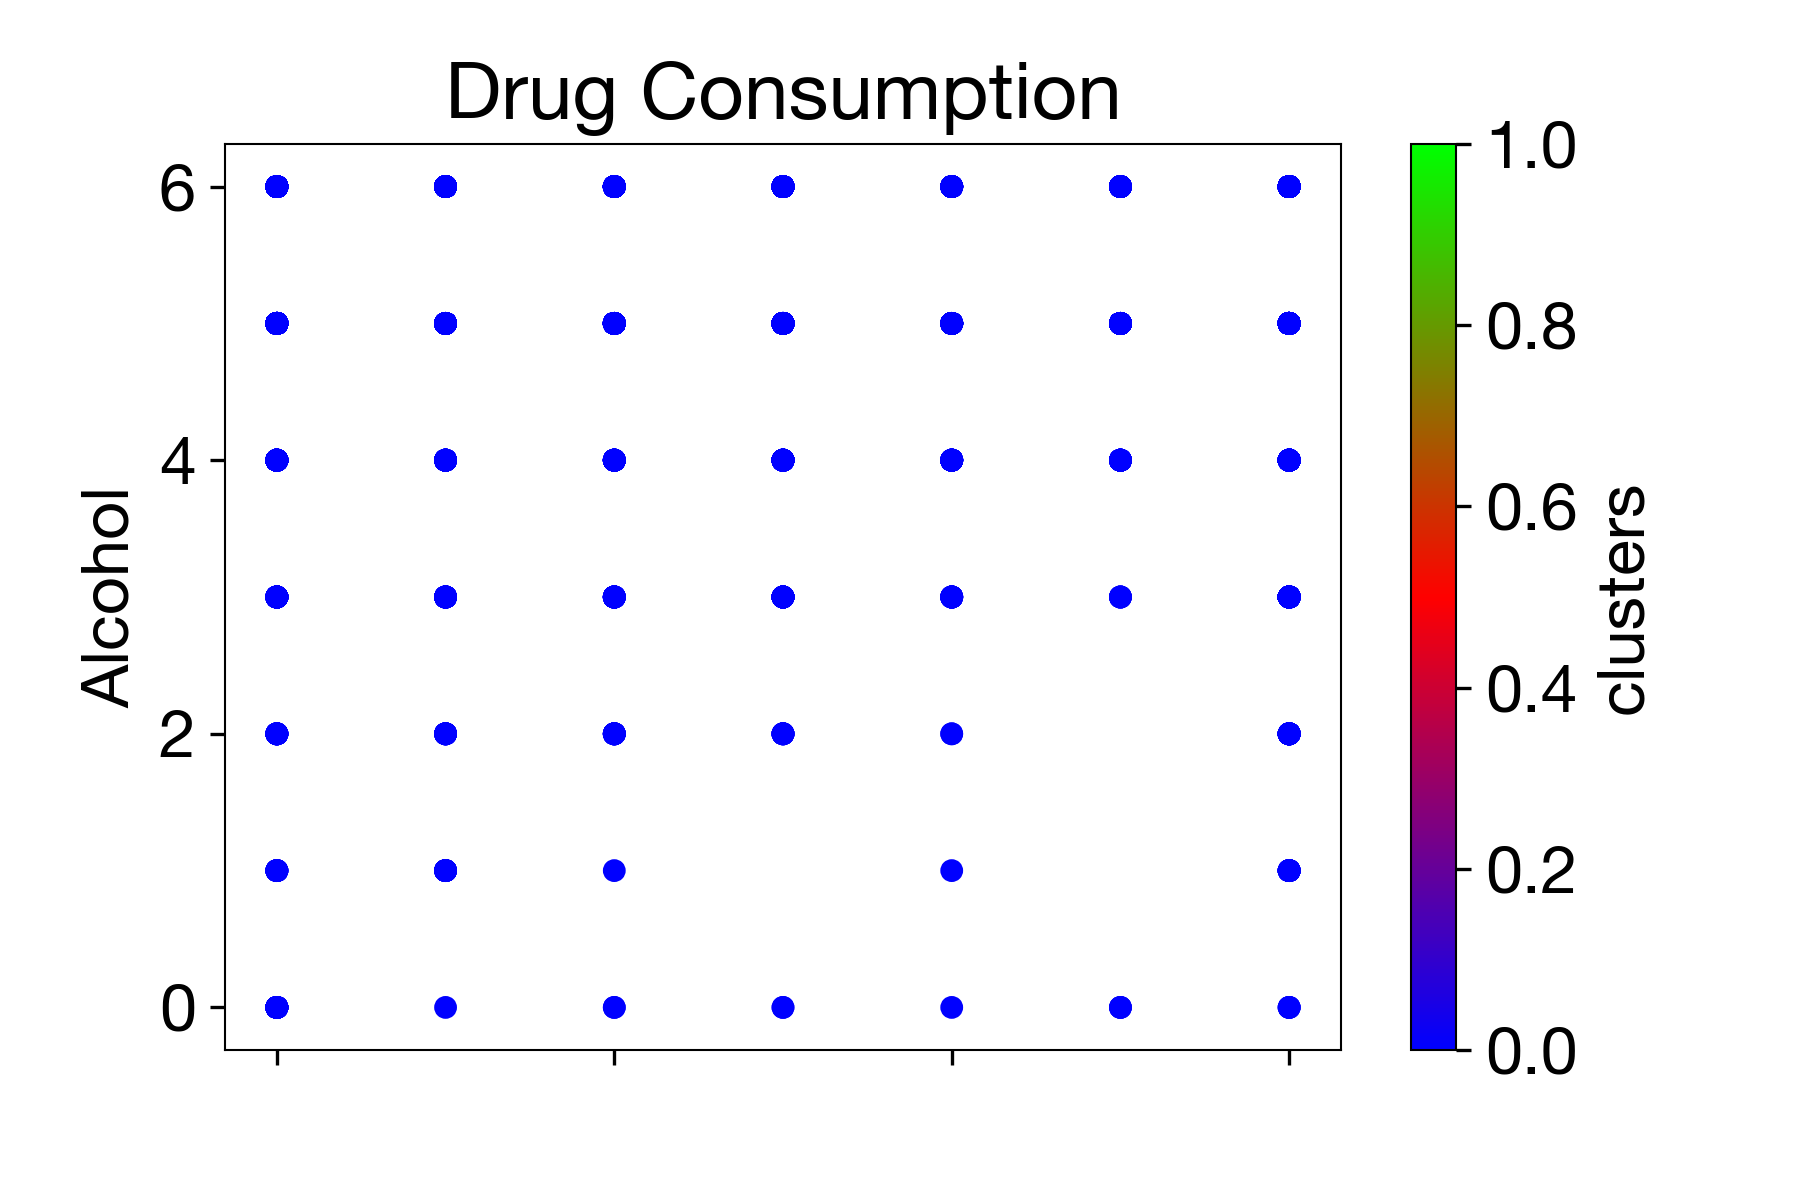
\includegraphics[scale=0.35]{cluster2-NicotineVsAlcohol.png}
\end{figure}

\begin{figure}[H]
\caption{Cluster with all features(Ascore VS Coke) }
\label{fig:AscoreVsCoke}
\centering
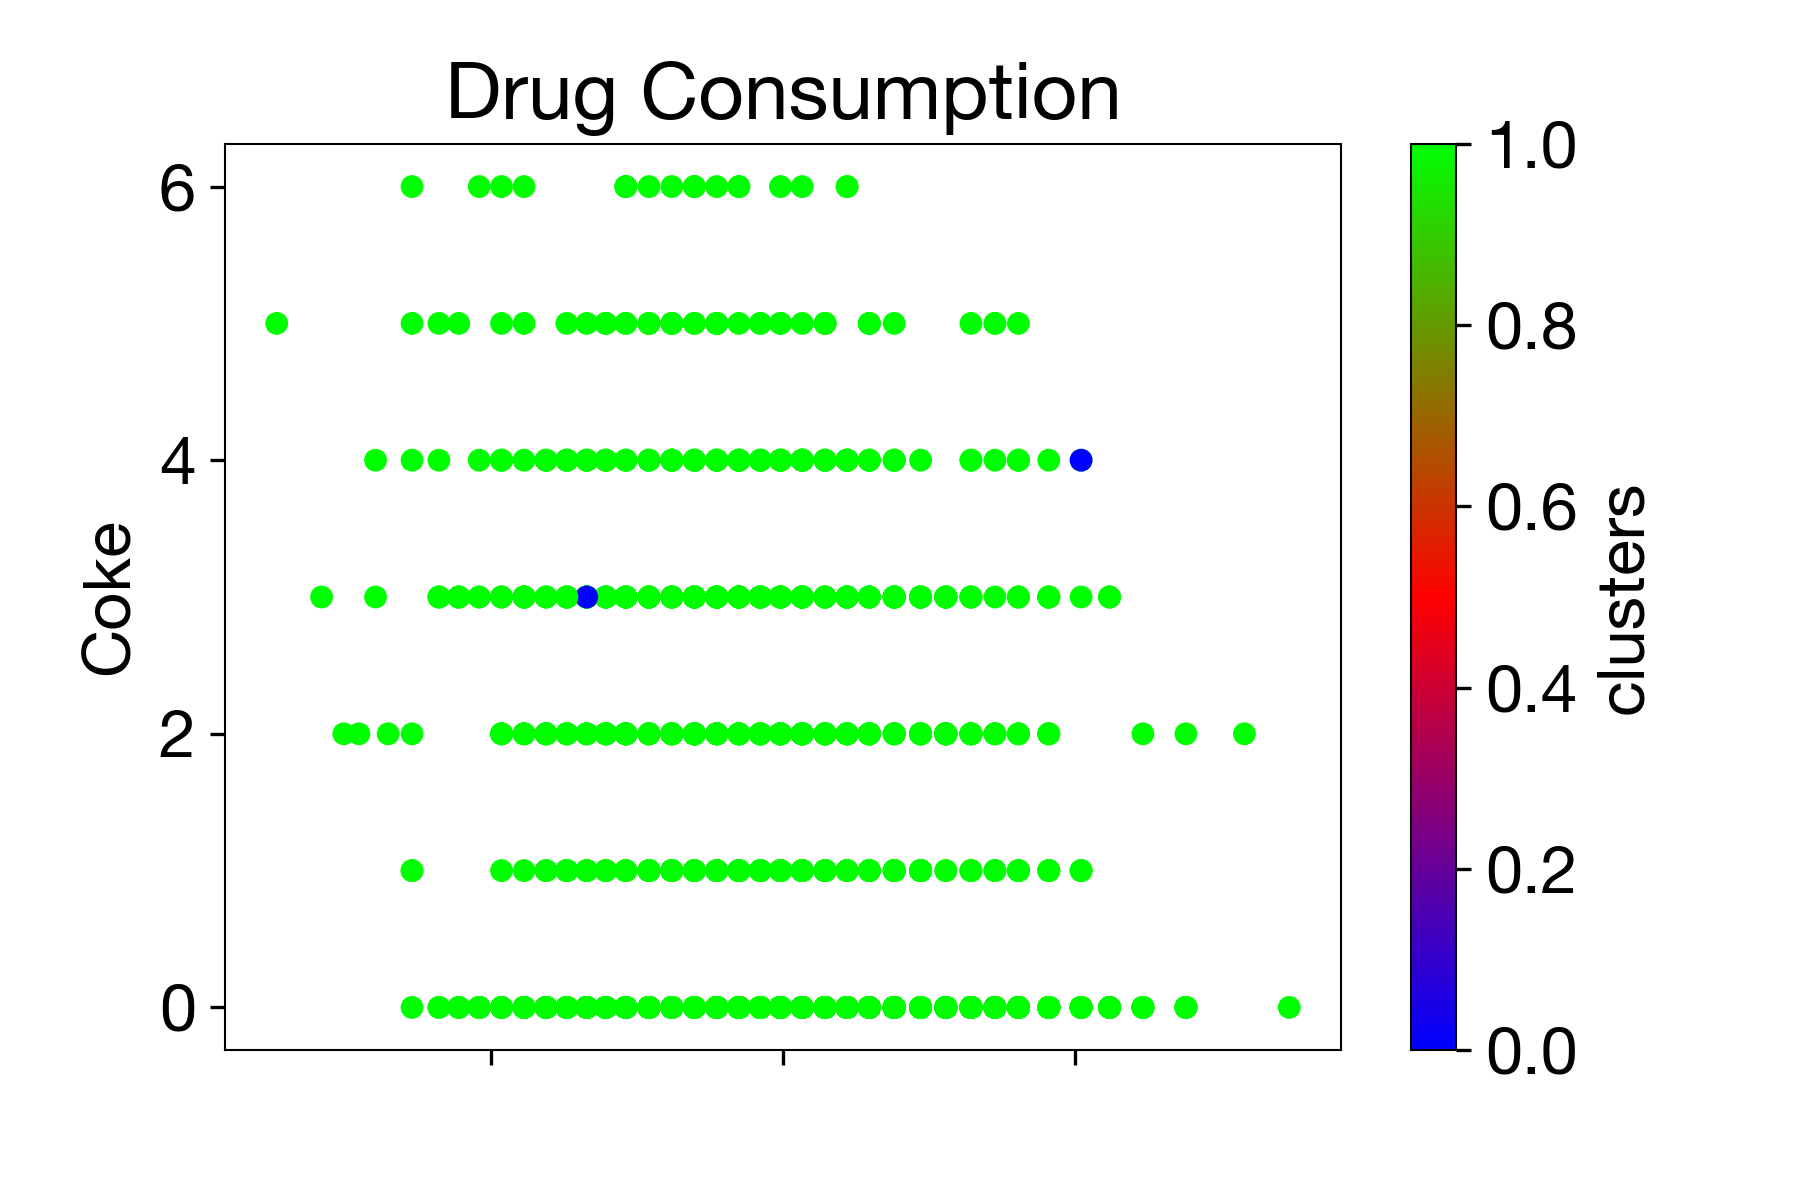
\includegraphics[scale=0.35]{cluster1-AscorevsCoke.png}
\end{figure}

\begin{figure}[H]
\caption{Cluster with All features excluding drugs(Ascore VS Nscore) }
\label{fig:AscoreVSNscore}
\centering
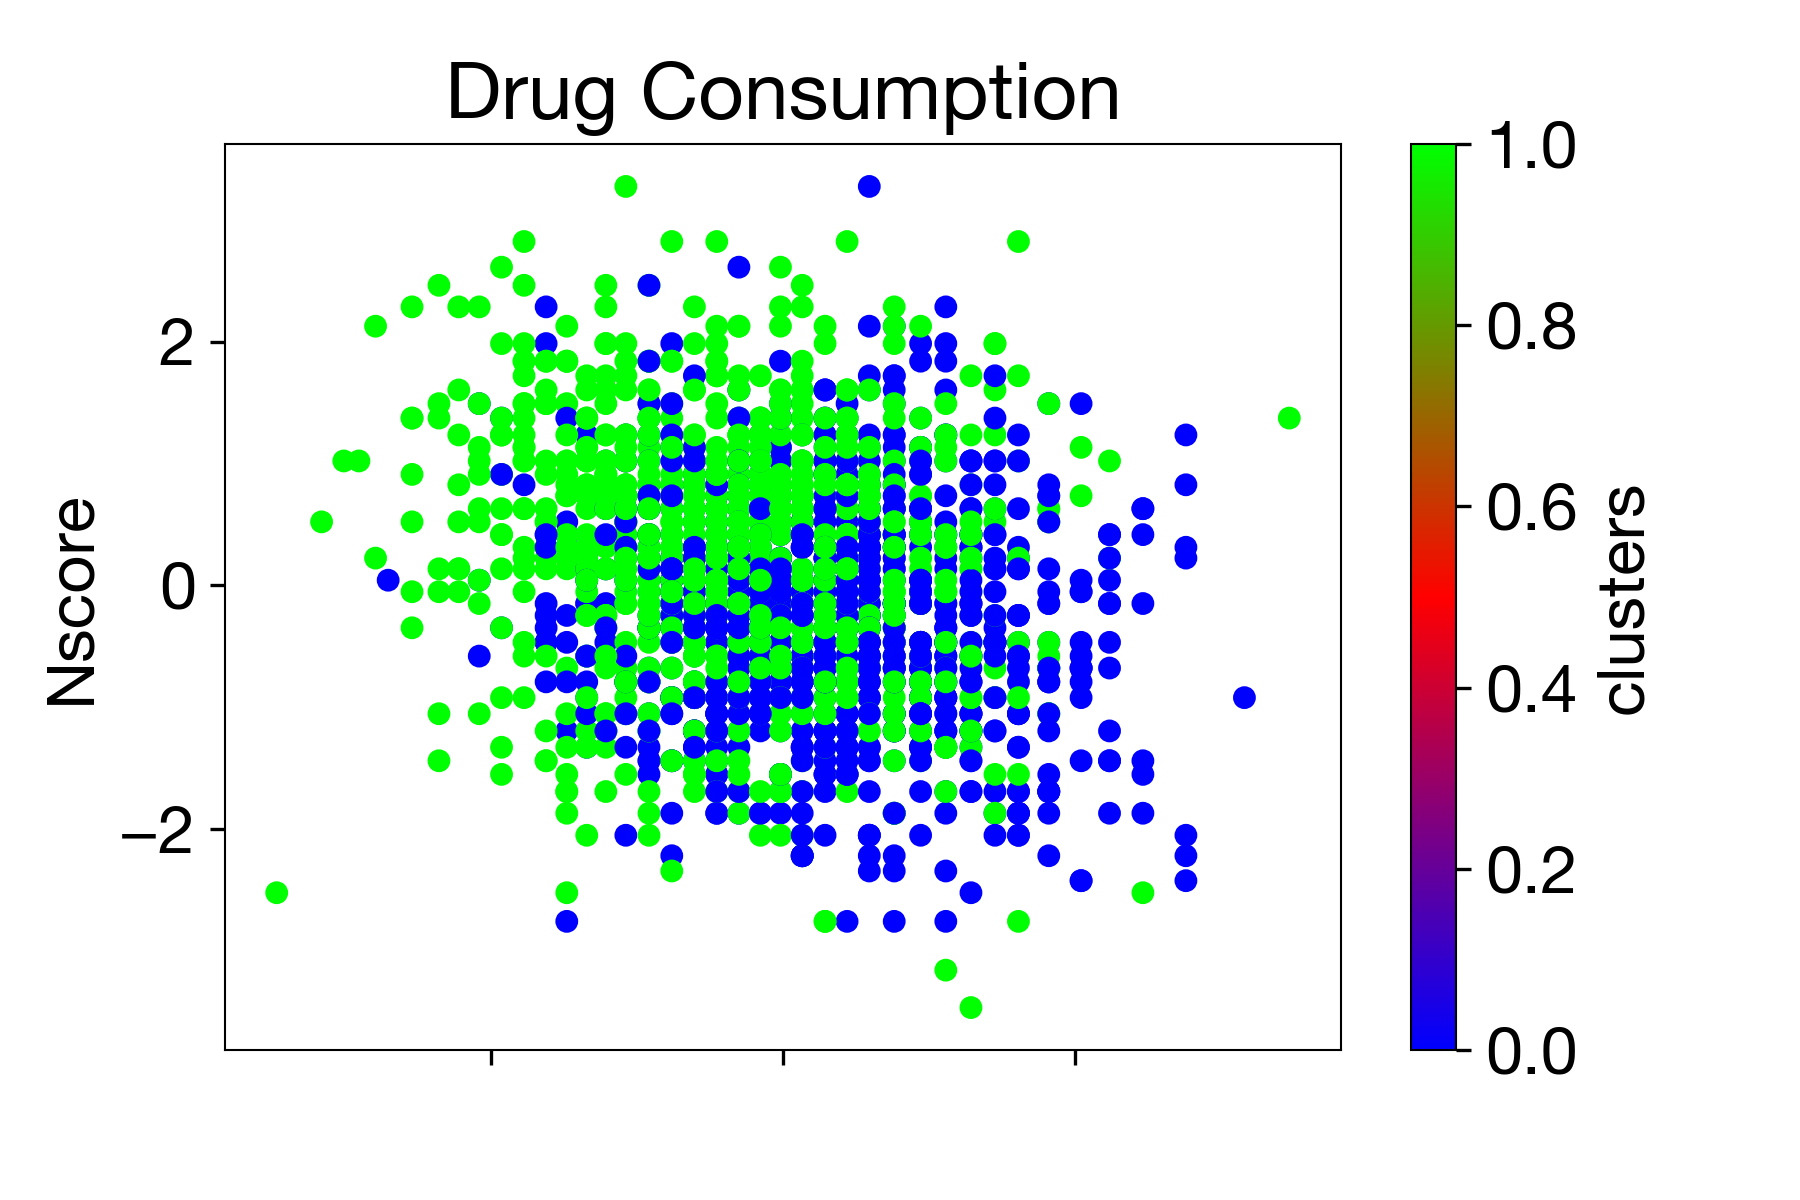
\includegraphics[scale=0.35]{cluster5-AscoreVsNscore.png}
\end{figure}

\begin{figure}[H]
\caption{Cluster with only Personality Traits(Oscore VS Impulsive) }
\label{fig:OscoreVSImpulsive}
\centering
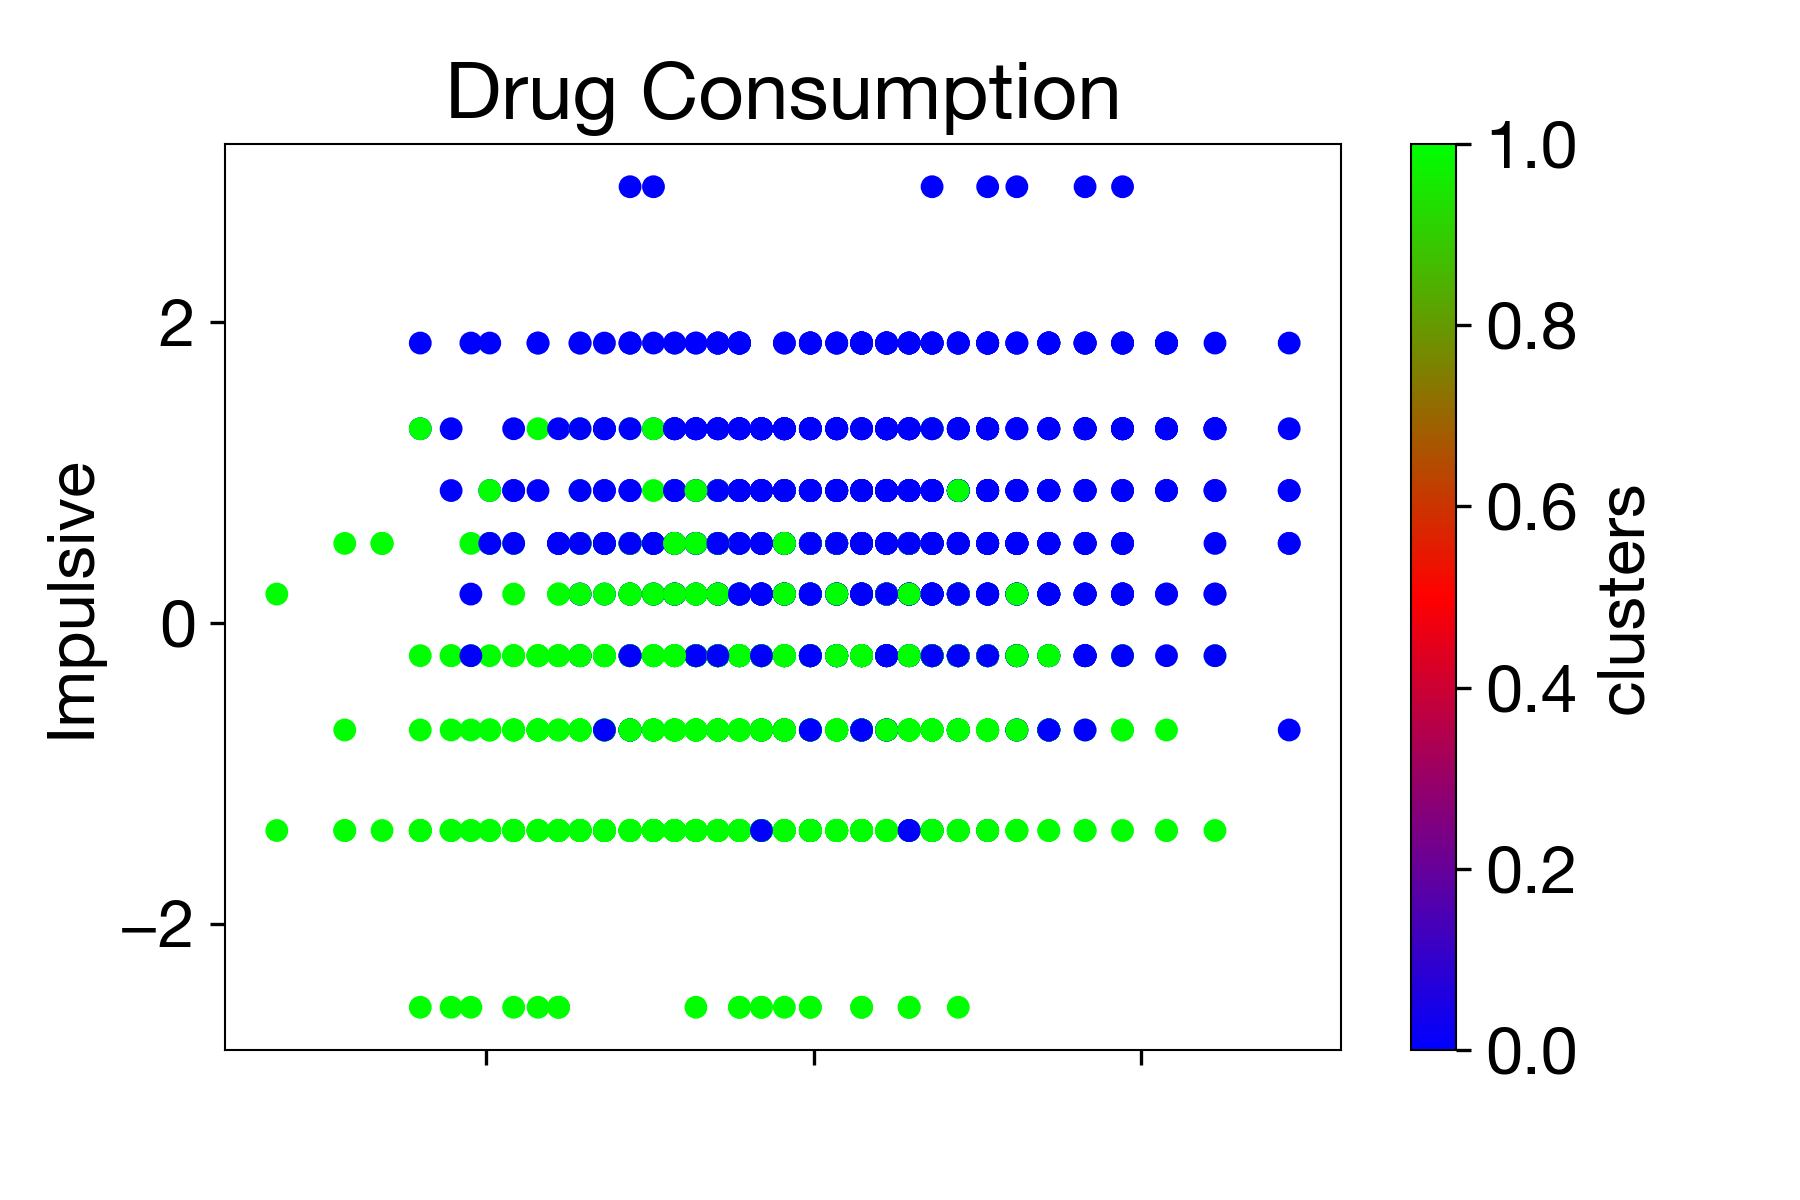
\includegraphics[scale=0.35]{cluster6-OscoreVImpulsive.png}
\end{figure}

    After the plotting, we realized that there aren't any clusters which gives a significant view into the relationship between the features. We did try to plot the clusters with drug features having binary values, but that resulted in even worse clusters. 
    
    
\section*{6. Results}

	Summarizing all the silhouette coefficients of clusters resulted in the following table. From the table, it can be clearly observed that the clusters that are made up of Only Illegal, Only Non-Illegal and Only Drugs have the highest Silhouette Coefficient which means they are good clusters compared to the others. And, we can also see the performance of each clustering technique.
 \begin{figure}[H]
\caption{Silhouette Coefficients of Various Clusters }
\label{fig:SilhouetteCoeff}
\centering
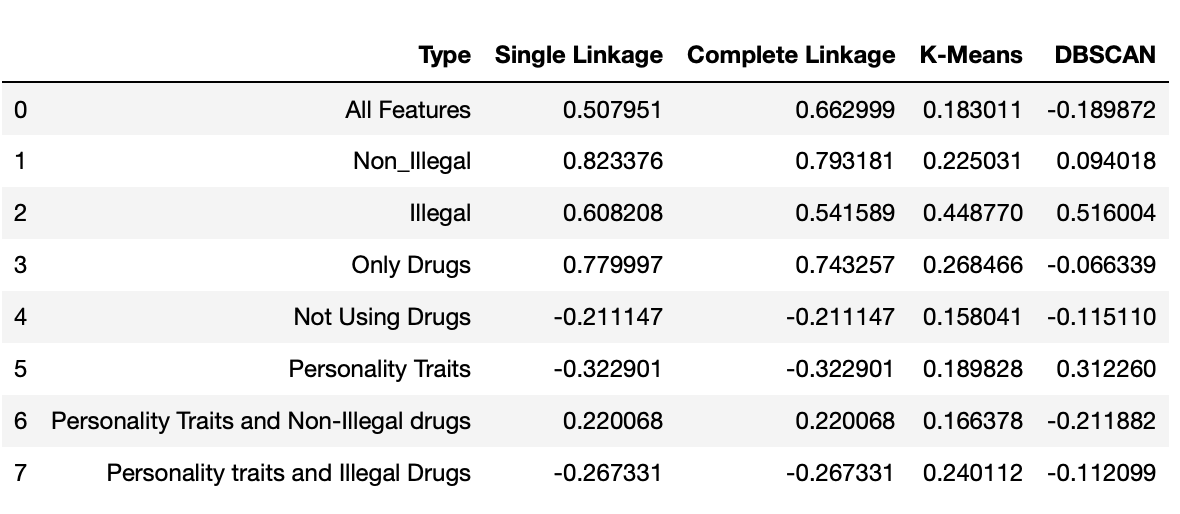
\includegraphics[scale=0.5]{Cluster_Table.png}
\end{figure}

The best performing binary classifier was the random forest classifier with a mean accuracy of 91.2\% when tested with 10-fold cross validation. On the test set, it had an accuracy of 82.7\% and an F1 score of 90.2\%. For the binary classifiers an obstacle they had to overcome was the large class imbalance caused by the popularity of cannabis in this dataset. Over 78\% of respondents have used cannabis at some time in their lives. We are not surprised that the random forest outperformed the decision tree on this dataset as the likelihood for overfitting seems high. We are satisfied with our model's ability to predict drug usage by using personality traits and other characteristics.
    
\end{document}
